\chapter{模擬データによる定量評価 \label{chapMock}}
% 3.1 模擬データの生成方法
% 3.2 解析方法
%  3.2.1 ベイズ推定の基礎
%  3.2.2 解析に用いる尤度関数
% 3.3 模擬データを用いた定量評価の結果
%  3.3.1 asymmetric driftの影響 (今、メールでは名称を省略しています)
%  3.3.2 ...影響
%  3.3.7 ...影響
% 3.4 解析結果のまとめ


% Chap. 3 模擬データ解析結果
% じっくり議論しながら整理したほうがよいので、
% また火曜日に議論しましょう。とりあえず、まだ書いていない 3.3.6、3.3.7も書いてみてください。


本論文では、オールト定数と太陽運動を測定する上で実際の銀河系速度場を反映しない値を得てしまう可能性があることから、模擬データによる定量評価とその結果を踏まえた観測データ解析を行い正確なオールト定数と太陽運動の測定を目指す。観測データの解析では、解析結果の値が正しいのか間違っているのか、つまり実際の銀河系速度場を表した値なのかどうかを判断できない。なぜなら、当然ではあるが観測データ解析においては答えが分かっていないからである。そこで、観測データの代わりに解析に用いるモデルを利用して模擬データを生成し、それを解析する。それによって、正しい答え、すなわち模擬データのセッティングパラメータと解析結果のパラメータ値とを比較することができる。

位置・速度の6次元位相空間情報を持つ模擬データを生成し、それを解析することで、asymmetric drift、視線速度情報を用いる解析と用いない解析、速度楕円体の傾き、太陽からの距離$D$、円盤面からの距離$|z|$、太陽と銀河中心との距離$R_{\odot}$のそれぞれの解析への影響を定量的に評価した。この章では模擬データの生成方法と解析結果についてまとめる。

\section{模擬データの生成方法}
観測方程式(\ref{ObsEq})に従う速度場を仮定し、密度分布には指数関数的密度分布$\rho(R,z) = \rho_0 e^{-R/h_R} e^{-z/h_z}、h_R=3\,\mathrm{kpc}、h_z=300\,\mathrm{pc}$\,(\cite{BH2016})を仮定している。ここで、$R,z$はそれぞれ円筒座標系での動径方向と鉛直方向の位置、$h_R、h_z$は$R、z$方向の密度分布のスケール長を示す。サンプル数は基本的に1000とし、太陽からの距離$D<1\,\mathrm{kpc}$としている。このときの3次元分布と1次元の頻度分布太陽の銀河中心からの距離は$R_{\odot} = 8.2\,\mathrm{kpc}$(\cite{BH2016})としている。また、asymmetric drift速度には式(\ref{AD3})を使用する。

解析1から解析6までの6パターンで解析を行っている。解析1から解析5までの解析では、模擬データの生成に表\ref{table4}のようなパラメータセットを使用している。表\ref{table6}は本論文で生成した模擬データのデータセットである。asymmetric driftを模擬データで考慮するかしないか、速度楕円体の傾きの角度、サンプル星の太陽からの距離の最大値、サンプル星の円盤面からの距離の最大値を変更して複数の種類のデータを生成している。表\ref{VelocityDispersion}は\cite{YL18}で調べられた年齢速度分散関係の表であり、今回の模擬データ生成では表\ref{VelocityDispersion}の年齢速度分散関係を仮定している。

\begin{table}
\begin{center}
%\scalebox{0.5}
%\scriptsize
%\footnotesize
%\small
\begin{tabular}{l|c} \hline
 \rowcolor{LightCyan}
 パラメータ & 値\\
 \hline
 $A$ & 18 $\mathrm{km\,s^{-1} kpc^{-1}}$\\
 \hline
 $B$ & -11 $\mathrm{km\,s^{-1} kpc^{-1}}$\\
 \hline
 $C$ & -2 $\mathrm{km\,s^{-1} kpc^{-1}}$\\
 \hline
 $K$ & -1 $\mathrm{km\,s^{-1} kpc^{-1}}$\\
 \hline
 $U_{\odot}$ & 9 $\mathrm{km\,s^{-1}}$\\
 \hline
 $V_{\odot}$ & 11 $\mathrm{km\,s^{-1}}$\\
 \hline
 $W_{\odot}$ & 7.5 $\mathrm{km\,s^{-1}}$\\
 \hline
 $R_{\odot}$ & 8.2 $\mathrm{kpc}$\\
 \hline
\end{tabular}
\vspace{3mm}
\caption{模擬データ生成で用いた各パラメータの設定値。}
\label{table4}
\end{center}
\end{table}

\begin{table}
\begin{center}
%\scalebox{0.5}
%\scriptsize
%\footnotesize
%\small
\begin{tabular}{c|c|c|c|c} \hline
 \rowcolor{LightCyan}
 データ名 & ADあり/なし & VE & $D_{\mathrm{max}}\,(\si{kpc})$ & $z_{\mathrm{max}}\,(\si{kpc})$\\
 \hline
 A & $\bigcirc$ & $0^{\circ}$ & 1 & 1\\
 \hline
 B & $\times$ & $0^{\circ}$ & 1 & 1\\
 \hline
 B-VE20 & $\times$ & $20^{\circ}$ & 1 & 1\\
 \hline
 B-VE40 & $\times$ & $40^{\circ}$ & 1 & 1\\
 \hline
 B-D03 & $\times$ & $0^{\circ}$ & 0.3 & 1\\
 \hline
 B-D06 & $\times$ & $0^{\circ}$ & 0.6 & 1\\
 \hline
 B-z01 & $\times$ & $0^{\circ}$ & 1 & 0.1\\
 \hline
 B-z03 & $\times$ & $0^{\circ}$ & 1 & 0.3\\
 \hline
\end{tabular}
\vspace{3mm}
\caption{生成した模擬データセット。ADはasymmetric drift、VEは速度楕円体 (velocity ellipsoid)、$D_{\mathrm{max}}$はサンプル星の太陽からの距離の最大値、$z_{\mathrm{max}}$はサンプル星の円盤面からの距離の最大値のことである。サンプル数は全て$10^3$、太陽と銀河中心との距離は全て$R_{\odot}=8.2\,\si{kpc}$としている。}
\label{table6}
\end{center}
\end{table}

\begin{table}
\begin{center}
%\scalebox{0.5}
%\scriptsize
%\footnotesize
%\small
\begin{tabular}{c|c|c|c} \hline
 \rowcolor{LightCyan}
 星の年齢 $\tau\,\mathrm{(Gyr)}$ & $\sigma_R\,\mathrm{(km\ s^{-1})}$ & $\sigma_{\phi}\,\mathrm{(km\ s^{-1})}$ & $\sigma_{z}\,\mathrm{(km\ s^{-1})}$\\
 \hline
 1.4 & 21.7 & 12.0 & 8.6\\
 \hline
 1.9 & 21.4 & 16.7 & 10.1\\
 \hline
 2.4 & 27.8 & 18.9 & 10.5\\
 \hline
 2.8 & 32.7 & 18.4 & 11.0\\
 \hline
 3.3 & 31.3 & 16.8 & 11.9\\
 \hline
 3.8 & 30.1 & 16.9 & 11.7\\
 \hline
 4.3 & 34.7 & 17.8 & 12.6\\
 \hline
 4.9 & 36.8 & 21.2 & 16.8\\
 \hline
 5.6 & 39.3 & 22.1 & 17.7\\
 \hline
 6.4 & 42.5 & 23.0 & 18.3\\
 \hline
 7.2 & 43.8 & 24.2 & 23.3\\
 \hline
 8.5 & 51.8 & 25.8 & 23.3\\
 \hline
\end{tabular} \label{VelocityDispersion}
\vspace{3mm}
\caption{模擬データ生成で用いた年齢と速度分散の対応表 (\cite{YL18})。速度分散は銀河中心を中心とした円筒座標系$(R,\phi,z)$となっている。}
\end{center}
\end{table}

図\ref{dist3dMockData}、\ref{distMockData}は以上のパラメータセットで生成したサンプル数1000での模擬データの3次元分布と頻度分布である。頻度分布の方を見ると、サンプル数が1000個のためランダム性が排除できていないが、指数関数的密度分布$\rho(R,z) = \rho_0 e^{-R/h_R} e^{-z/h_z}$にしたがっていることがわかる。

%\subsection{模擬データの生成コード}
%以下に模擬データの作成コードのうちの1つを記述する。このコードではexponential diskを仮定し、太陽からの距離1kpc以内に1000個の星があるとしている。OLCODモデルに従った速度場を持たせている。
%\lstinputlisting[language=Python]{code/MockGenerate.py}


\begin{figure*}[htbp]
\begin{center}
	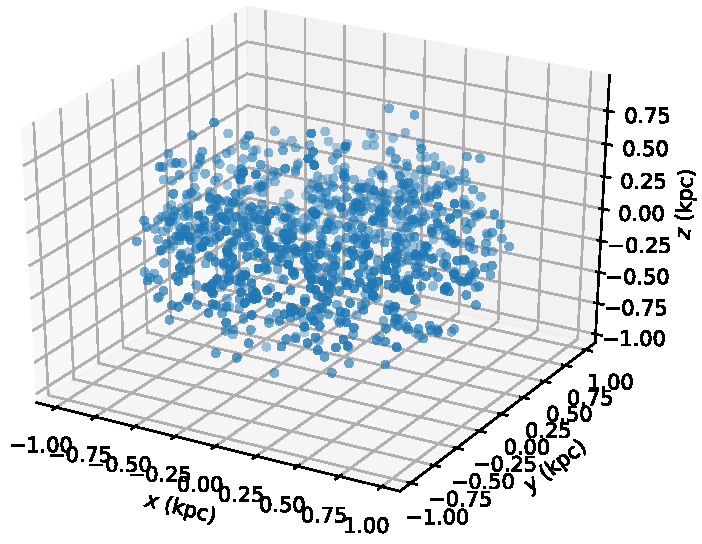
\includegraphics[width=9cm]{fig/3dMockData.pdf}
	\caption{1000個の星の模擬データの3次元分布}
	\label{dist3dMockData}
\end{center}
\end{figure*}

\begin{figure*}
   \centering
\begin{tabular}{ccc}
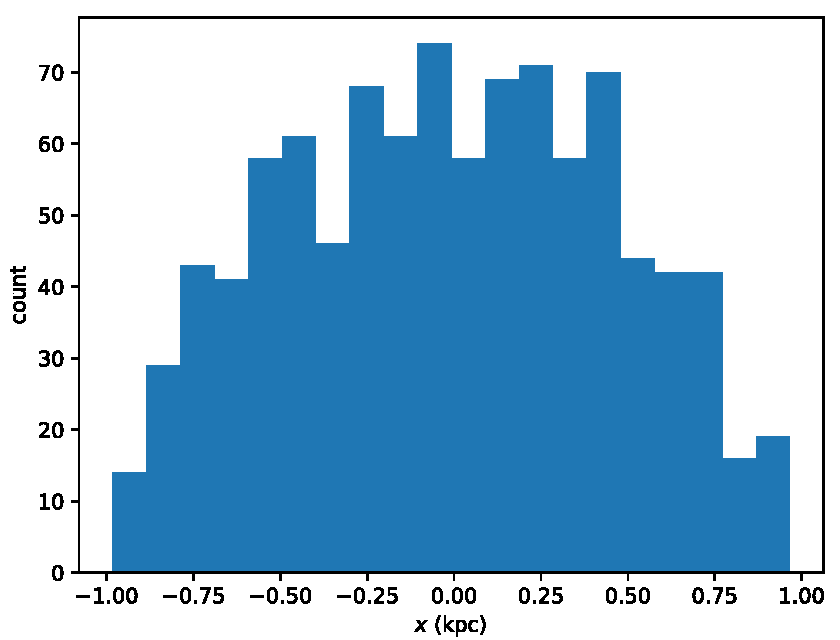
\includegraphics[width=4.5cm]{fig/dist_x.pdf}&
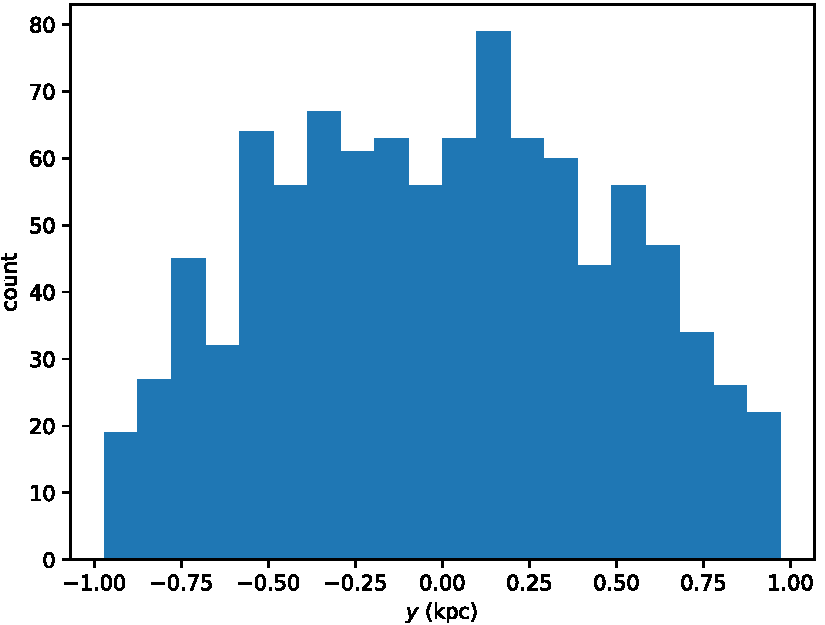
\includegraphics[width=4.5cm]{fig/dist_y.pdf}&
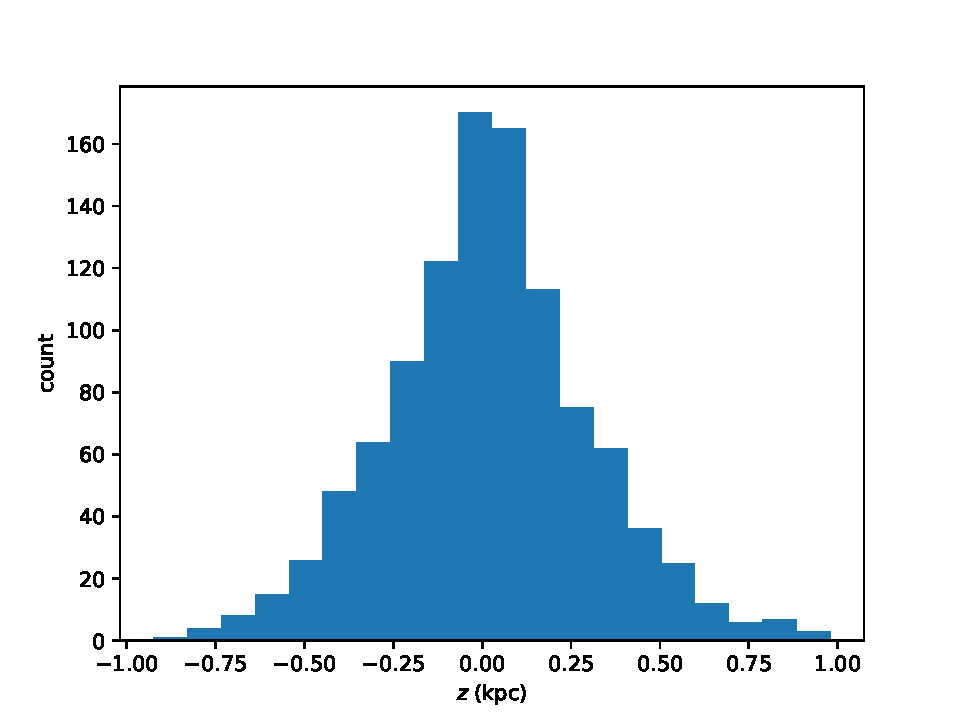
\includegraphics[width=4.5cm]{fig/dist_z.pdf}
\end{tabular}
    \caption{1000個の星の模擬データの頻度分布。$x、y、z$は太陽を原点とした直交座標系の軸の向きで、それぞれ銀河中心方向、銀河回転方向、銀河北極方向である。左の図から順に横軸は$x、y、z$、縦軸はそれぞれの値の範囲である。ビンは100 pcごとにしている。}
    \label{distMockData}
\end{figure*}

%%%%%%%%%%%%%%%%%%%%%%%%%%%%%%%%%%%%%%%%%%%%%%%%%%%%%%%%%%%%%%%%%%%%%%%%%%%%%%%%%%%%
%%%%%%%%%%%%%%%%%%%%%%%%%%%%%%%%%%%%%%%%%%%%%%%%%%%%%%%%%%%%%%%%%%%%%%%%%%%%%%%%%%%%

\section{解析方法}
この節では、第\ref{chapTheory}章を踏まえてデータの解析方法を説明する。まず本研究の解析で用いているベイズ推定について簡単に説明し、その後解析で使用している式や仮定について説明する。本論文では模擬データの生成と解析を6パターン行っており、それぞれの解析結果の詳細は\ref{模擬データの解析結果}で記述する。本節では、6パターンに共通する解析の基本的な部分を説明する。解析方法を大まかに分けると、asymmetric driftを考慮した場合と考慮しない場合とに分けられるため、この2パターンの解析方法については本節で説明する。

\subsection{ベイズ推定の基礎 \label{ベイズ推定の基礎}}
本研究では解析にベイズ推定(Bayesian Estimation)を用いるため、\cite{Statictics2012}に基づいてベイズ推定について説明する。

あるランダムな事象$A$は0と1の間の確率prob$(A)$を持っているとする。この事象$A$が確実に起こるとき、$\mathrm{prob}(A)=1$となる。また、事象$A$と事象$B$が相互に排他的なとき、すなわち同時に起こらないとき、$\mathrm{prob}(A\,\mathrm{or}\,B)=\mathrm{prob}(A) + \mathrm{prob}(B)$となる。これはコルモゴロフの公理 (Kolmogorov axiom)と呼ばれる。

この2つの事象$A、B$はの一方の確率がもう一方の確率に影響しないとき、$A、B$は独立であるという。このとき、コルモゴロフの公理から$\mathrm{prob}(A\,\mathrm{and}\,B)=\mathrm{prob}(A)\,\mathrm{prob}(B)$と書ける。しかし、時には独立が保たれないことがある。このときには条件付き確率というものを考える。条件$B$の下での$A$の条件付き確率は
\begin{align}
\begin{aligned}
	\mathrm{prob}(A|B) = \frac{\mathrm{prob}(A\,\mathrm{and}\,B)}{\mathrm{prob}(B)}
\end{aligned}
\end{align}
と定義される。このとき、
\begin{align}
\begin{aligned}
	\mathrm{prob}(B|A) &= \frac{\mathrm{prob}(A\,\mathrm{and}\,B)}{\mathrm{prob}(B)}\\
	&= \mathrm{prob}(A|B)\,\frac{\mathrm{prob}(B)}{\mathrm{prob}(A)}\\
	&= \frac{\mathrm{prob}(A|B)\mathrm{prob}(B)}{\mathrm{prob}(A)}
\end{aligned} \label{Bayesian}
\end{align}
と書け、この式はベイズの定理と呼ばれる。$\mathrm{prob}(B)$はデータが得られる前の想定されている確率であり、事前確率 (prior probability)と呼ばれる。この経験というものは尤度$\mathrm{prob}(A|B)$で表され、ある状況での尤もらしさを示す。最後に$\mathrm{prob}(B|A)$は事後確率 (posterior probability)と呼ばれ、データを用いて事前確率を修正した結果の確率である。

ベイズ推定とは、ベイズ学習を繰り返すことで何らかのパラメータを推定する手法のことである。そこで、ベイズ学習について説明する。まず、ベイズの定理 (式(\ref{Bayesian}))と事前確率、尤度を用いて事後確率を計算したとする。さらにもう一度式(\ref{Bayesian})で計算しようとするとき、1回目の計算で得られた事後確率は2回目の事前確率として使用され、新たな事後確率が得られる。このように事後確率を更新していくことをベイズ学習と呼ぶ。

一般的にベイズ推定がパラメータ推定に用いられる際には、ここまでの説明に出てきた確率は単なる1つの値ではなく確率分布として与えられることが多く、本研究でも確率分布として扱う。さらに、尤度はあるパラメータに関する関数、すなわち尤度関数として用いる。尤度関数とは、あるデータが与えられたときに、そのデータの値の尤もらしさを出力する関数のことである。ベイズ学習の中で確率$\mathrm{prob}(A)$が変わらないとき、式(\ref{Bayesian})から
\begin{align}
\begin{aligned}
	\mathrm{prob}(B|A) \propto \mathrm{prob}(A|B)
\end{aligned}
\end{align}
と書けるため、ベイズ推定では一般的に尤度関数が重要な要素となる。

パラメータ推定法として広く使われる最尤推定法 (Maximum Likelihood Estimation)は事前確率に一様分布を仮定しており尤度だけから真の値を推定するが、ベイズ推定では任意の事前分布をかけている。すると、$一様分布\times 尤度関数$の確率分布の最頻値 (尤度関数の最大値)が最尤推定量となる。一方ベイズ推定では1つの値ではなく確率分布で与えられることから、パラメータを1つの値としてではなく確率分布として得たい場合には、ベイズ推定を用いることが好ましい。

ベイズ推定として最も広く使われる解析手法がマルコフ連鎖モンテカルロ法(Markov chain Monte Carlo methods; MCMC)である。マルコフ連鎖を利用したモンテカルロ法を用いると、データの分布を計算せずに直接事後分布を求めることができる。マルコフ連鎖(Markov chain)とは、ひとつのステップの中で前のパラメータの尤度に基づいて次のパラメータを決めることをいう。また一般に、乱数を用いた計算アルゴリズムをモンテカルロ法(Monte Carlo method)と呼ぶ(モンテカルロがカジノで有名なためにこう名付けられたという。ラスベガス法という別の方法も存在する)。

モンテカルロ法では真にランダムにサンプリングを行うため、
\begin{itemize}
	\item{計算コストがかさむ}
	\item{精度が向上しない}
\end{itemize}
という課題がある。計算コストがかさむ理由は、MCMCはマルコフ連鎖を利用していることから、限られた範囲で乱数発生をすればよいのに対し、モンテカルロ法のみの場合には毎ステップでマルコフ連鎖を利用する場合に比べて広範囲の乱数発生をしなくてはならず、その分計算コストが大きくなるためである。精度が向上しない理由は、マルコフ連鎖を利用しない場合には広範囲で乱数発生をしなければならないが、その際に乱数をあまり細かくすると計算コストが膨大になるため、広範囲な乱数を発生する代償として乱数は粗くなることになり、結果的に得られる確率分布の精度は悪くなる。MCMCは、マルコフ連鎖を定常分布としたサンプリングを行うことで、上記の課題を改善した方法である。

MCMCのアルゴリズムは以下の通りである。
\begin{enumerate}
	\item{初期点を決める}
	\item{マルコフ連鎖により次のサンプリングを行う分布を決定する}
	\item{分布が収束をするまで、(2)を繰り返す}
\end{enumerate}
基本的なアルゴリズムはこのようなものであるが、さらに具体的なアルゴリズムには高速化や精度の向上を目指していくつかの方法が開発されており、それらの一部に付録で触れることとする。本研究では、MCMCの解析に天文学研究で広く使われているemcee (\cite{Foreman2013}) を使用している。


%%%%%%%%%%%%%%%%%%%%%%%%%%%%%%%%%%%%%%%%%%%%%%%%%%%%%%%%%%%%%%%%%%%%%%%%%%%%%%%%%%%%
%%%%%%%%%%%%%%%%%%%%%%%%%%%%%%%%%%%%%%%%%%%%%%%%%%%%%%%%%%%%%%%%%%%%%%%%%%%%%%%%%%%%

\subsection{解析に用いる尤度関数 \label{解析に用いる尤度関数}}
MCMCによる解析では尤度関数を定義する必要がある。ここでは、本研究の解析で用いているフィッティングパラメータと尤度関数についての説明を行う。

\subsubsection{(a) asymmetric driftを考慮しない場合}
フィッティングパラメータは$A、B、C、K、U_{\odot}、V_{\odot}、W_{\odot}、\sigma_{\mu_l}、\sigma_{\mu_b}、\sigma_{v_{\mathrm{los}}}$の10個である。このときの尤度関数を求める。$\sigma_{\mu_l}、\sigma_{\mu_b}、\sigma_{v_{\mathrm{los}}}$はそれぞれ$\mu_l、\mu_b、v_{\mathrm{los}}$の平均速度場からの速度分散を表す。このとき尤度関数$\mathcal{L}$は
\begin{align}
\begin{aligned}
	\ln \mathcal{L} =& -\frac{1}{2}\sum_i \left(\frac{\left[\mu_{l,i} - \mu_l^{\mathrm{OL}}(l_i,b_i,\varpi_i)\right]^2}{\sigma_{\mu_l}^2 + (s_{\mu_{l,i}})^2}  + {\rm ln}\left[\sigma_{\mu_l}^2 + (s_{\mu_{l,i}})^2\right] \right. \\
	&+ \left. \frac{\left[\mu_{b,i} - \mu_b^{\mathrm{OL}}(l_i,b_i,\varpi_i)\right]^2}{\sigma_{\mu_b}^2 + (s_{\mu_{b,i}})^2}  + {\rm ln}\left[\sigma_{\mu_b}^2 + (s_{\mu_{b,i}})^2\right] \right. \\
	&+ \left. \frac{\left[v_{\mathrm{los},i} - v^{\mathrm{OL}}_{\mathrm{los}}(l_i,b_i,\varpi_i)\right]^2}{\sigma_{v_{\mathrm{los}}}^2 + (s_{v_{\mathrm{los},i}})^2} + {\rm ln}\left[\sigma_{v_{\mathrm{los}}}^2 + (s_{v_{\mathrm{los},i}})^2\right] \right)
\end{aligned} \label{Likelihood_Mock}
\end{align}
と書ける。ここで、添字の$i$は$i$番目の星の値であることを示し、この添字があるパラメータは観測量である。また、$s_{\mu_{l,i}}、s_{\mu_{b,i}}、s_{v_{\mathrm{los},i}}$はそれぞれ$\mu_{l,i},\mu_{b,i},v_{\mathrm{los},i}$の観測誤差である。また、$\mu_l^{\mathrm{OL}}、\mu_b^{\mathrm{OL}}、v^{\mathrm{OL}}_{\mathrm{los}}$には\ref{観測方程式}の式(\ref{ObsEq})を用いている。

\subsubsection{(b) asymmetric driftを考慮する場合 \label{asymmetric driftを考慮する場合}}
フィッティングパラメータは同様に$A、B、C、K、U_{\odot}、V_{\odot}、W_{\odot}、\sigma_{\mu_l}、\sigma_{\mu_b}、\sigma_{v_{\mathrm{los}}}$の10個である。asymmetric driftを考慮する解析では、尤度関数$\mathcal{L}$には
\begin{align}
\begin{aligned}
	\ln \mathcal{L} =& -\frac{1}{2}\sum_i \left(\frac{\left[\mu_{l,i} - \mu_l^{\mathrm{AD}}(l_i,b_i,\varpi_i)\right]^2}{\sigma_{\mu_l}^2 + (s_{\mu_{l,i}})^2}  + {\rm ln}\left[\sigma_{\mu_l}^2 + (s_{\mu_{l,i}})^2\right] \right. \\
	&+ \left. \frac{\left[\mu_{b,i} - \mu_b^{\mathrm{AD}}(l_i,b_i,\varpi_i)\right]^2}{\sigma_{\mu_b}^2 + (s_{\mu_{b,i}})^2}  + {\rm ln}\left[\sigma_{\mu_b}^2 + (s_{\mu_{b,i}})^2\right] \right. \\
	&+ \left. \frac{\left[v_{\mathrm{los},i} - v^{\mathrm{AD}}_{\mathrm{los}}(l_i,b_i,\varpi_i)\right]^2}{\sigma_{v_{\mathrm{los}}}^2 + (s_{v_{\mathrm{los},i}})^2} + {\rm ln}\left[\sigma_{v_{\mathrm{los}}}^2 + (s_{v_{\mathrm{los},i}})^2\right] \right)
\end{aligned} \label{Likelihood_Mock_AD}
\end{align}
を使う。ここで、添字の$i$は$i$番目の星の値であることを示し、この添字があるパラメータは観測量である。ADの添字が付いているモデルの式についてはを参照。この式の中の$\mu_l^{\mathrm{AD}}、\mu_b^{\mathrm{AD}}、v^{\mathrm{AD}}_{\mathrm{los}}$には式(\ref{ObsEqAD})を用いている。$\mu_l^{\mathrm{AD}}、\mu_b^{\mathrm{AD}}、v^{\mathrm{AD}}_{\mathrm{los}}$の中でasymmetric drift速度$v_{\mathrm{a}}$を用い、さらに$v_{\mathrm{a}}$には式(\ref{AD3})の$v_{\mathrm{a}}=\sigma^2_R/80\,\si{km.s^{-1}}$を採用する。この$v_{\mathrm{a}}$を求めるために$\sigma_R$を計算する必要があるため、以下では観測量から$\sigma_R$を得る上の過程を説明する。まず以下の式でその準備を行う。
\begin{align}
\begin{aligned}
	D_i &= \varpi_i^{-1},\\
	R_i &= \sqrt{D_i^2 + R_{\odot}^2 - 2D_iR_{\odot}\cos{l_i}},\\
	\sin{\phi_i} &= \dfrac{D_i}{R_i}\sin{l_i},\\
	\cos{\phi_i} &= \sqrt{1 - \sin^2{\phi_i}},
\end{aligned} \label{eq142}
\end{align}
$D_i、R_i、l_i、\phi_i$については図(\ref{coor_a})を参照。
\begin{figure*}
	\centering
	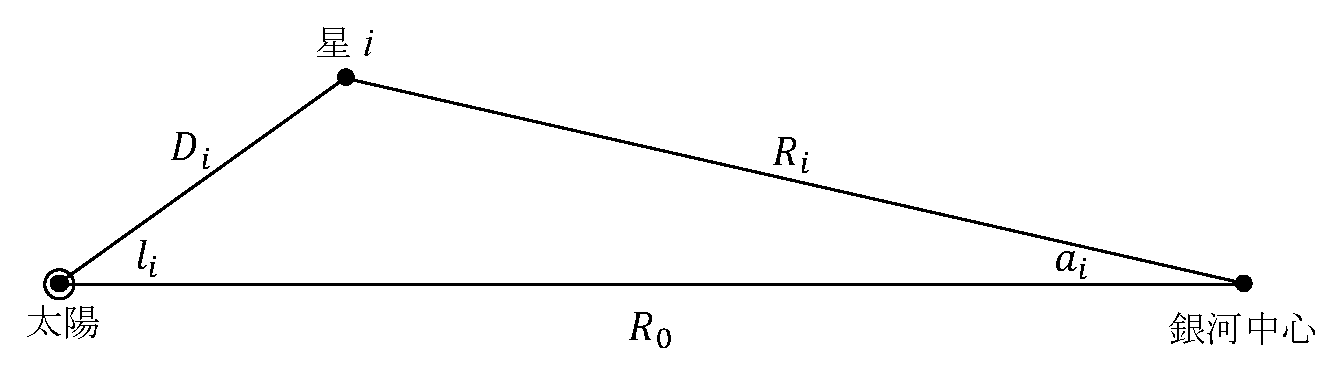
\includegraphics[width=10cm]{fig/coordinate_a2.pdf}
	\caption{星$i$と太陽、銀河中心の間のそれぞれの距離と角度の名称の定義。}
	\label{coor_a}
\end{figure*}

asymmetric driftを考慮するために、銀河中心を静止基準とするときの星と太陽の速度が必要となる。$v_R$の平均値$\overline{v_R}=0$という仮定を用いると、式(\ref{eq2.5})から
\begin{align}
	A - B =& \frac{1}{2}\left( \frac{V_{\phi}}{R_{\odot}} - \frac{\partial V_{\phi}}{\partial R} - \frac{1}{R_{\odot}}\frac{\partial v_{R}}{\partial \phi} \right)_{R=R_{\odot}} - 
	\frac{1}{2}\left( -\frac{V_{\phi}}{R_{\odot}} - \frac{\partial V_{\phi}}{\partial R} + \frac{1}{R_{\odot}}\frac{\partial v_{R}}{\partial \phi} \right)_{R=R_{\odot}}\\
	=& \frac{V_{\phi}}{R_{\odot}} - \frac{1}{R_{\odot}}\frac{\partial v_{R}}{\partial \phi} \\
	=& \frac{V_{\phi}}{R_{\odot}}
\end{align}
であるから、
\begin{align}
	V_{\mathrm{\phi}} = R_{\odot}(A-B) \label{eq153}
\end{align}
と表せる。また、接線速度は
\begin{align}
\begin{aligned}
	v_{l,i} =& \mu_{l,i}D_i \kappa\\
	v_{b,i} =& \mu_{b,i}D_i \kappa
\end{aligned}
\end{align}
と表せる。ここで、$\kappa=4.74047\,\si{km.s^{-1}.kpc^{-1}/(.mas.yr^{-1})}$は単位変換に用いられる定数である。円筒座標系の速度は
\begin{align}
\begin{aligned}
	\left(
	\begin{array}{c}
	 	v_{R,i}\\
		v_{\phi,i}\\
		v_{\mathrm{los},i}
	\end{array}
	\right)
	=& \bf{Q}^{\mathrm{T}} \left[\bf{P}^{\mathrm{T}}
	\left(
	\begin{array}{c}
	 	v_{l,i}\\
		v_{b,i}\\
		v_{\mathrm{los},i}
	\end{array}
	\right)
	+\left(
	\begin{array}{c}
	 	U_{\odot}\\
		V_{\odot} + V_{\mathrm{\phi}}\\
		W_{\odot}
	\end{array}
	\right)
	\right]
\end{aligned}
\end{align}
と変換される。ここから、$v_R$の標準偏差$\sigma_R$は
\begin{align}
\begin{aligned}
	\sigma_R = \sqrt{\frac{1}{N}\sum^N_i(v_{R,i} - \frac{1}{N}\sum^N_i v_{R,i})^2}
\end{aligned}
\end{align}
と計算できる。ここで、$N$はサンプル星の数である。このasymmetric drift速度を銀河座標系に変換すると
\begin{align}
\begin{aligned}
	\left(
	\begin{array}{c}
	 	v_{a,l}\\
		v_{a,b}\\
		v_{a,\mathrm{los}}
	\end{array}
	\right)
	=& \bf{P} \bf{Q}
	\left(
	\begin{array}{c}
	 	0\\
		v_a\\
		0
	\end{array}
	\right)
\end{aligned}
\end{align}
のようになる。表記法は\ref{sec_ObsAD}と同様である。

%%%%%%%%%%%%%%%%%%%%%%%%%%%%%%%%%%%%%%%%%%%%%%%%%%%%%%%%%%%%%%%%%%%%%%%%%%%%%%%%
%%%%%%%%%%%%%%%%%%%%%%%%%%%%%%%%%%%%%%%%%%%%%%%%%%%%%%%%%%%%%%%%%%%%%%%%%%%%%%%%
%%%%%%%%%%%%%%%%%%%%%%%%%%%%%%%%%%%%%%%%%%%%%%%%%%%%%%%%%%%%%%%%%%%%%%%%%%%%%%%%

\section{模擬データの解析結果 \label{模擬データの解析結果}}
模擬データの解析では表\ref{table5}で書いているようにasymmetric drift、視線速度情報を用いる状況と用いない状況、速度楕円体の傾き、太陽からの距離、円盤面からの距離、サンプル数、太陽の銀河中心からの距離$R_{\odot}$の6つの効果を考える解析パターンで、模擬データ生成あるいは解析方法を変更してオールト解析における効果を調べた。表\ref{table4}、\ref{table5}はそれぞれの解析で用いた模擬データの設定と仮定を示している。asymmetric driftについては解析に際して入れる必要がある場合のみ模擬データに入れている。また、太陽は円盤面上に位置していると仮定している。$R_{\odot}$の効果を調べる理由は、先行研究で使われている$R_{\odot}$の値がだいたい$\SI{7.5}{kpc}$から$\SI{8.5}{kpc}$の間でばらつきがあり一定ではないため、仮定する$R_{\odot}$の値が解析に大きな影響を及ぼさないかどうか調べたいためである。

MCMCの設定について説明する。初期値は表\ref{table4}の値のプラスマイナス5の範囲で一様に乱数を振って生成している。また、walkerは60、iterationは2000とし、burn-inは1000としている。walkerとはほぼ独立して尤度関数にしたがってパラメータ空間内を動いていく点のことである。iterationとは、MCMCのランダムサンプリングをする回数のことである。burn-inとは、MCMCのある時点までのサンプリング結果を捨てることであり、burn-inが1000、iterationが2000という場合には、サンプリング回数2000のうち最初の1000は捨てるということである。これは、MCMCによるパラメータ推定はすぐには収束しないことから、収束するまでのサンプリング結果は最終的な推定値の確率分布の計算には含めないためである。今回の模擬データ解析では、総じてサンプリング1000ではサンプリングに収束が見えたため、burn-inを1000としている。また、乱数を降るときの大きさ (proposal scale parameter)は2となっている。つまり、あるパラメータのある時点での推定値が10となっているとき、尤度を計算するために生成する次の値は9.8あるいは10.2となる。

表\ref{table5}で試行回数について書いているが、この場合の試行回数とはすなわち模擬データ1を生成してそれを解析する、模擬データ2を生成してそれをまた解析する、という風に、試行回数が例えば10の場合には模擬データ1から模擬データ10までの10個の模擬データを生成してそれぞれを全く同様に解析するという意味である。最終的な解析結果には、試行回数分の結果の値の平均値を使用する。模擬データのサンプル数は全て1000としている。これは、1000個のサンプルならばある程度の精度が得られ、かつ計算時間も長すぎないという都合からである。なお、1000サンプルでも各解析結果の評価にポアソンノイズが影響してしまうため、乱数のシードを変えた模擬データを10個生成し、それぞれを解析して10個の解析結果の平均値を使用している。

また、それぞれの解析結果で各パラメータの相対誤差fit-trueと絶対誤差$\log_{10}\left| \dfrac{\mathrm{fit} - \mathrm{true}}{\mathrm{true}}\right|$をプロットしているが、相対誤差の絶対値の大きさの順番と絶対誤差の大きさの順番は必ずしも一致しない。なぜなら、相対誤差を計算するときには試行回数分の解析ごとの相対誤差を足しているので、例えばtrueの値が1の場合に試行1の相対誤差が1で試行2の相対誤差が-1だった場合でこの2回の平均値を考えると、相対誤差は$[1+(-1)]/2=0$となる一方、絶対誤差は$[|1|+|-1|]/2=1$となり、複数の解析結果の平均値を使用しているために相対誤差の絶対値をとったものが絶対誤差になる訳ではない。

\begin{table}
\begin{center}
%\scalebox{0.5}
%\scriptsize
%\footnotesize
%\small
\begin{tabular}{l|c|c} \hline
 \rowcolor{LightCyan}
 解析名 & 模擬データにAD & 尤度関数にAD \\
 \hline
 解析1: asymmetric driftの解析結果への影響 &$\bigcirc$& $\bigcirc$\\
 \hline
 解析2: 視線速度の有無による解析結果への影響 & $\times$ & $\times$\\
 \hline
 解析3: 速度楕円体の傾きの解析結果への影響 & $\times$ & $\times$\\
 \hline
 解析4: 太陽からの距離の解析結果への影響 & $\times$ & $\times$\\
 \hline
 解析5: 円盤面からの距離の解析結果への影響 & $\times$ & $\times$\\
 \hline
 解析6: $R_{\odot}$の値の解析結果への影響 & $\bigcirc$ & $\bigcirc$\\
 \hline
\end{tabular}
\vspace{3mm}
\caption{それぞれの解析で用いた設定。asymmetric driftの有無は、模擬データにasymmetric driftを入れたか入れないかを示している。試行回数は、模擬データを同じ設定値で生成し解析したパターン数。これは、ランダム性を可能な限り解消するためにいくつかのパターンで同じセッティングでのデータ生成を行って、全パターンの解析で得られた値の平均値を解析結果として用いている。}
\label{table5}
\end{center}
\end{table}

%%%%%%%%%%%%%%%%%%%%%%%%%%%%%%%%%%%%%%%%%%%%%%%%%%%%%%%%%%%%%%%%%%%%%%%%%%%%%%%%%%%%%%%%%%%%%%%%
%%%%%%%%%%%%%%%%%%%%%%%%%%%%%%%%%%%%%%%%%%%%%%%%%%%%%%%%%%%%%%%%%%%%%%%%%%%%%%%%%%%%%%%%%%%%%%%%
%%%%%%%%%%%%%%%%%%%%%%%%%%%%%%%%%%%%%%%%%%%%%%%%%%%%%%%%%%%%%%%%%%%%%%%%%%%%%%%%%%%%%%%%%%%%%%%%

\subsection{解析1: asymmetric driftの解析結果への影響}
asymmetric driftの効果を入れた模擬データAについて、asymmetric driftを考慮しない解析(観測方程式(\ref{ObsEq}))とasymmetric driftを考慮した解析(観測方程式(\ref{ObsEqAD}))との2通りの解析を行う。asymmetric drift $v_{\mathrm{a}}$は、表の$\sigma_R$と式(\ref{AD3})から計算して$v_{\phi}\to v_{\phi}-v_{\mathrm{a}}$のようにして各年齢ごとに異なる値を入れる。図(\ref{fig:Mock_AD})はこの模擬データの解析結果である。asymmetric drift無しと有りでは、$A、B、V_{\odot}$で明らかな違いがあり、総じてasymmetric drift有り (with AD)はfitとtrueとの差が0に近いのに対し、asymmetric drift無し (no AD)ではfitがtrieに対して差を持っている。特に$V_{\odot}$では、星のどの年齢においてもfitの値がtrueの値よりも大きくなっている。また、年齢が大きくなるほどfitとtrueとの差が大きくなり、最大で$\SI{35}{km.s^{-1}}$大きくなっている。$A$では、年齢が大きくなるほどno ADのfitがtrueに比べて小さくなっている。$B$は8 Gyrを除いて年齢が大きくなるほどno ADのfitがtrueに比べて大きくなっている。with ADの方は、$A$、$B$共にほぼfitとtrueとが一致しているが、$B$は年齢が8.5 Gyrではno ADのfitの方がwith ADのfitよりもtrueに近い値となっている。

\begin{figure*}[htbp]
	\centering
	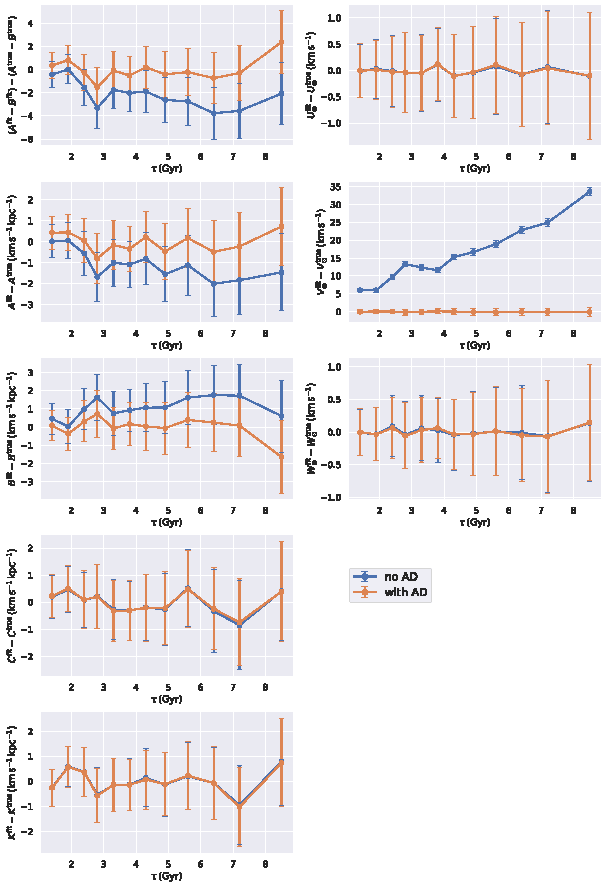
\includegraphics[width=15cm]{fig/Mock_AD.pdf}
	\caption{解析1。模擬データAをasymmetric driftを考慮せずに解析した結果 (オレンジ色)とasymmetric driftを考慮して解析した結果 (青色)。縦軸は各パラメータのfit (解析で得られた値) - true (模擬データに設定した値)、横軸は模擬データに入れた速度分散に対応する年齢。} \label{fig:Mock_AD}
\end{figure*}

%%%%%%%%%%%%%%%%%%%%%%%%%%%%%%%%%%%%%%%%%%%%%%%%%%%%%%%%%%%%%%%%%%%%%%%%%%%%%%%%%%%%%%%%%%%%%%%%
%%%%%%%%%%%%%%%%%%%%%%%%%%%%%%%%%%%%%%%%%%%%%%%%%%%%%%%%%%%%%%%%%%%%%%%%%%%%%%%%%%%%%%%%%%%%%%%%
%%%%%%%%%%%%%%%%%%%%%%%%%%%%%%%%%%%%%%%%%%%%%%%%%%%%%%%%%%%%%%%%%%%%%%%%%%%%%%%%%%%%%%%%%%%%%%%%

\subsection{解析2: 視線速度の有無による解析結果への影響}
解析2では、模擬データBを視線速度情報を含めた尤度関数式(\ref{Likelihood_Mock})と含めない尤度関数
\begin{align}
\begin{aligned}
	\ln \mathcal{L} =& -\frac{1}{2}\sum_i \left(\frac{\left[\mu_{l,i} - \mu_l^{\mathrm{OL}}(l_i,b_i,\varpi_i)\right]^2}{\sigma_{\mu_l}^2 + (s_{\mu_{l,i}})^2}  + {\rm ln}\left[\sigma_{\mu_l}^2 + (s_{\mu_{l,i}})^2\right] \right. \\
	&+ \left. \frac{\left[\mu_{b,i} - \mu_b^{\mathrm{OL}}(l_i,b_i,\varpi_i)\right]^2}{\sigma_{\mu_b}^2 + (s_{\mu_{b,i}})^2}  + {\rm ln}\left[\sigma_{\mu_b}^2 + (s_{\mu_{b,i}})^2\right] \right)
\end{aligned}
\end{align}
とで解析した。解析においてasymmetric driftは考慮していない。図\ref{fig:Mock_vlos}はその解析結果のプロットである。 発散を表す$K$では視線速度情報を含めた尤度関数での解析 (with vlos)の方が、含めない尤度関数での解析 (without vlos)に比べてどの年齢でもfit - trueが0に近くなっている。with vlosの方は最大でfitとtrueとの差は$\SI{0.2}{km.s^{-1}.kpc^{-1}}$程度に留まるが、without vlosの方は最大$\SI{2.0}{km.s^{-1}.kpc^{-1}}$程度、平均ではだいたい$\SI{1.0}{km.s^{-1}.kpc^{-1}}$の差がある。$K$以外のパラメータではwithout vlosとwith vlosとで大きな差はないが、太陽運動の回転方向成分$V_{\odot}$は年齢$\SI{2.8}{Gyr}$以上ではwithout vlosよりもwith vlosの方が精度が高くなっている。

\begin{figure*}[htbp]
	\centering
	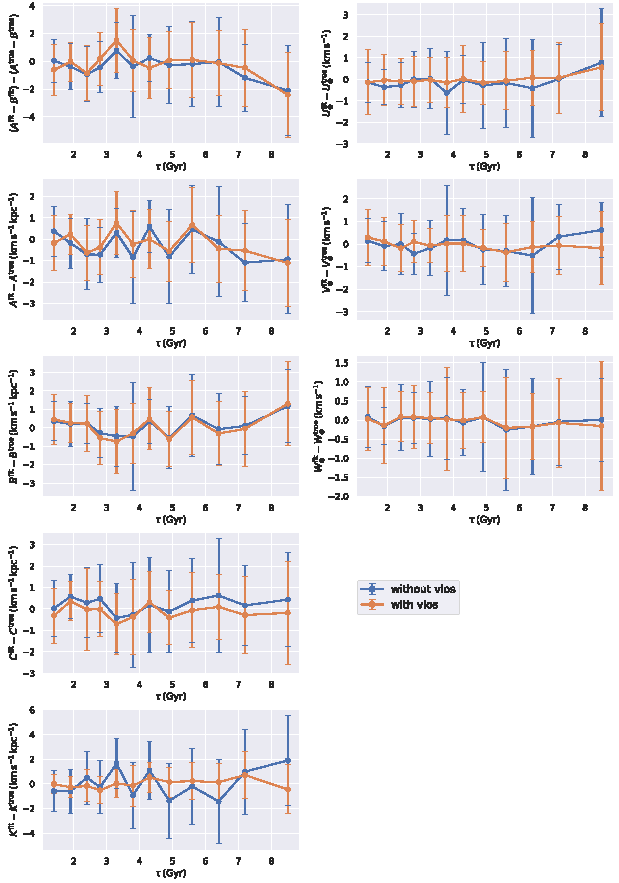
\includegraphics[width=15cm]{fig/Mock_vlos.pdf}
	\caption{解析2。模擬データBを視線速度情報を使用して解析した結果 (オレンジ色)と視線速度情報を使用せずに解析した結果 (青色)。解析にasymmetric driftは考慮していない。縦軸は各パラメータのfit (解析で得られた値) - true (模擬データに設定した値)、横軸は模擬データに入れた速度分散に対応する年齢。} \label{fig:Mock_vlos}
\end{figure*}

%%%%%%%%%%%%%%%%%%%%%%%%%%%%%%%%%%%%%%%%%%%%%%%%%%%%%%%%%%%%%%%%%%%%%%%%%%%%%%%%%%%%%%%%%%%%%%%%
%%%%%%%%%%%%%%%%%%%%%%%%%%%%%%%%%%%%%%%%%%%%%%%%%%%%%%%%%%%%%%%%%%%%%%%%%%%%%%%%%%%%%%%%%%%%%%%%
%%%%%%%%%%%%%%%%%%%%%%%%%%%%%%%%%%%%%%%%%%%%%%%%%%%%%%%%%%%%%%%%%%%%%%%%%%%%%%%%%%%%%%%%%%%%%%%%

\subsection{解析3: 速度楕円体の傾きの解析結果への影響 \label{解析3}}
模擬データB、B-VE20、B-VE40の3つの模擬データをそれぞれasymmetric driftを考慮せずに解析した。具体的には、速度$v_R$と$v_{\phi}$の間の速度楕円体の傾きを$l_{R\phi}$するとき、
\begin{align}
\begin{aligned}
	\left(
	\begin{array}{c}
	 	\sigma_{R,\mathrm{VE}}\\
	 	\sigma_{\phi,\mathrm{VE}}
	\end{array}
	\right)
	=
	\left(
	\begin{array}{cc}
	 	\cos{l_{R\phi}} & -\sin{l_{R\phi}}\\
	 	\sin{l_{R\phi}} & -\cos{l_{R\phi}}
	\end{array}
	\right)
	\left(
	\begin{array}{c}
	 	\sigma_R\\
	 	\sigma_{\phi}
	\end{array}
	\right)
\end{aligned}
\end{align}
のように$\sigma_R、\sigma_{\phi}$で描かれる速度楕円体を$l_{R\phi}$だけ回転させている。

図\ref{fig:Mock_VE}その解析結果である。この結果では、$l_{R\phi}$の値による大きな違いは見られない。

\begin{figure*}[htbp]
	\centering
	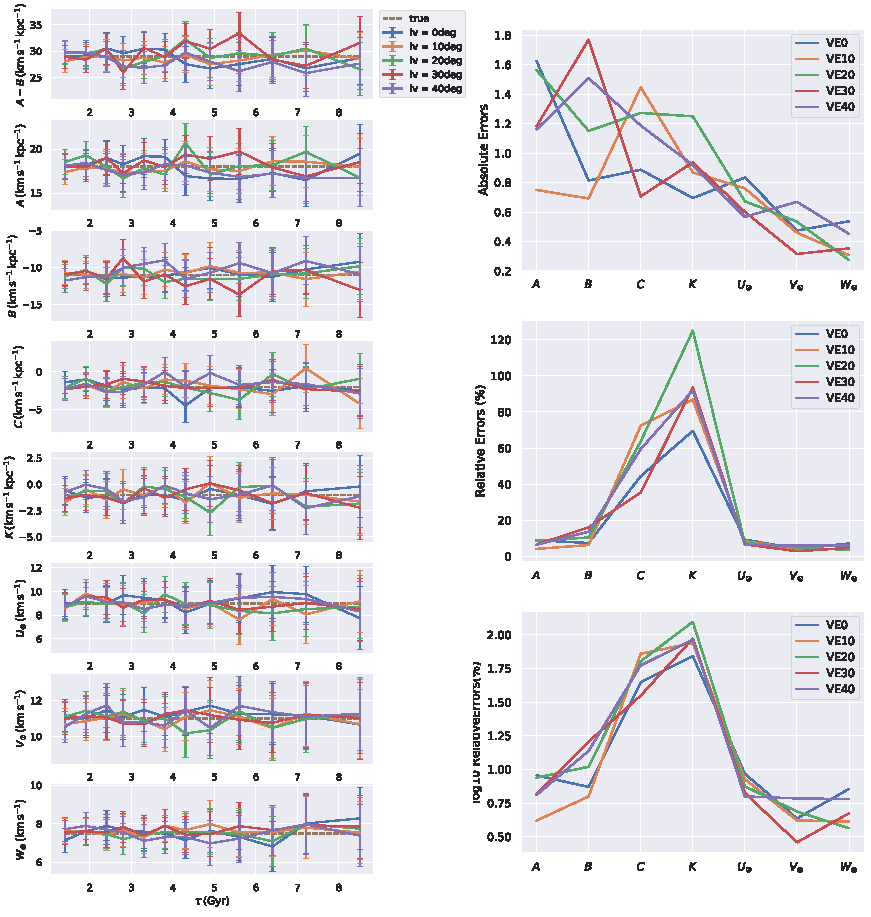
\includegraphics[width=15cm]{fig/Mock_VE.pdf}
	\caption{解析3。模擬データB、B-VE20、B-VE40をasymmetric driftを考慮せずに解析した結果。ラベルのlv = 0deg、20deg、40degはそれぞれ模擬データB、B-VE20、B-VE40の解析結果である。縦軸は各パラメータのfit (解析で得られた値) - true (模擬データに設定した値)、横軸は模擬データに入れた速度分散に対応する年齢。} \label{fig:Mock_VE}
\end{figure*}


%%%%%%%%%%%%%%%%%%%%%%%%%%%%%%%%%%%%%%%%%%%%%%%%%%%%%%%%%%%%%%%%%%%%%%%%%%%%%%%%%%%%%%%%%%%%%%%%
%%%%%%%%%%%%%%%%%%%%%%%%%%%%%%%%%%%%%%%%%%%%%%%%%%%%%%%%%%%%%%%%%%%%%%%%%%%%%%%%%%%%%%%%%%%%%%%%
%%%%%%%%%%%%%%%%%%%%%%%%%%%%%%%%%%%%%%%%%%%%%%%%%%%%%%%%%%%%%%%%%%%%%%%%%%%%%%%%%%%%%%%%%%%%%%%%

\subsection{解析4: 太陽からの距離の解析結果への影響}
解析4では、模擬データ模擬データB-D03、B-D06、Bをasymmetric driftを考慮せずに解析した。図\ref{fig:Mock_D}はその解析結果である。

B-D03の解析結果はB-D06、Bの解析結果に比べてどのパラメータもfitとtrueとの差が大きい。B-D06とBの解析結果ではfitとtrueとの差に大きな違いは見られない。また、年齢依存性は見られない。

\begin{figure*}[htbp]
	\centering
	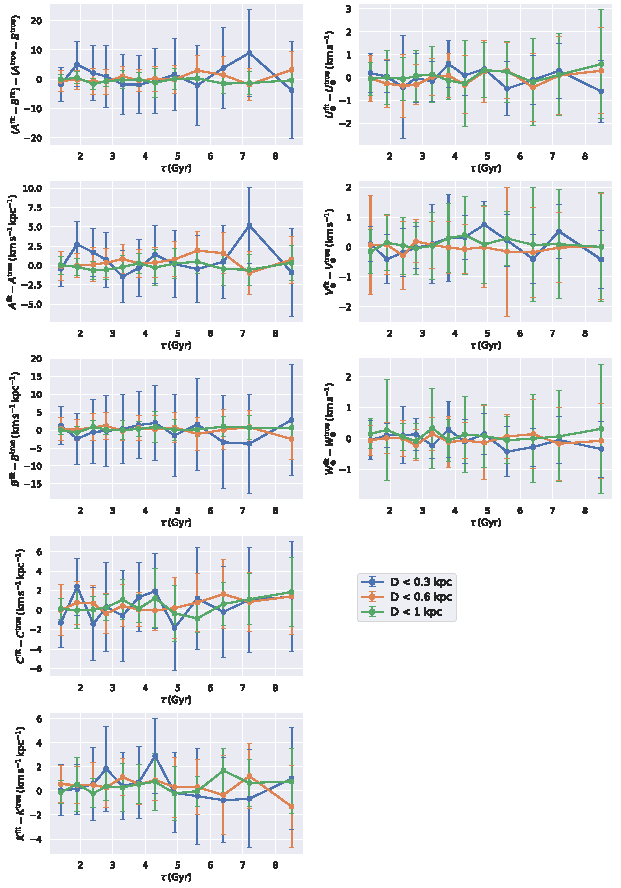
\includegraphics[width=15cm]{fig/Mock_D.pdf}
	\caption{解析4。模擬データB-D03、B-D06、Bをasymmetric driftを考慮せずに解析した結果。縦軸は各パラメータのfit (解析で得られた値) - true (模擬データに設定した値)、横軸は模擬データに入れた速度分散に対応する年齢。} \label{fig:Mock_D}
\end{figure*}

%%%%%%%%%%%%%%%%%%%%%%%%%%%%%%%%%%%%%%%%%%%%%%%%%%%%%%%%%%%%%%%%%%%%%%%%%%%%%%%%%%%%%%%%%%%%%%%%
%%%%%%%%%%%%%%%%%%%%%%%%%%%%%%%%%%%%%%%%%%%%%%%%%%%%%%%%%%%%%%%%%%%%%%%%%%%%%%%%%%%%%%%%%%%%%%%%
%%%%%%%%%%%%%%%%%%%%%%%%%%%%%%%%%%%%%%%%%%%%%%%%%%%%%%%%%%%%%%%%%%%%%%%%%%%%%%%%%%%%%%%%%%%%%%%%

\subsection{解析5: 円盤面からの距離の解析結果への影響}
解析5では模擬データB-z01、B-z03、Bをasymmetric driftを考慮せずに解析した。図\ref{fig:Mock_z}はその解析結果のプロットである。この解析結果からは$|z|$の値による大きな違いは見られず、それぞれの解析結果の値の違いはランダム性によるものだと考えられる。

\begin{figure*}[htbp]
	\centering
	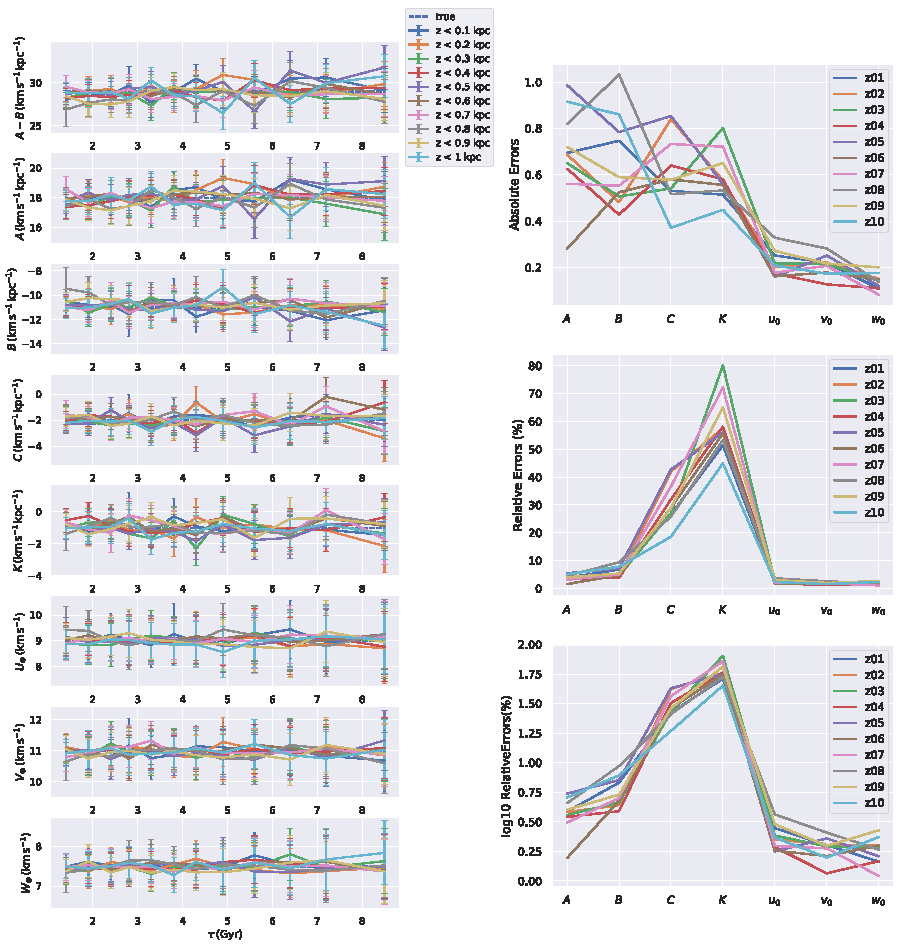
\includegraphics[width=15cm]{fig/Mock_z.pdf}
	\caption{解析5。模擬データB-z01、B-z03、Bをasymmetric driftを考慮せずに解析した結果。縦軸は各パラメータのfit (解析で得られた値) - true (模擬データに設定した値)、横軸は模擬データに入れた速度分散に対応する年齢。} \label{fig:Mock_z}
\end{figure*}

%%%%%%%%%%%%%%%%%%%%%%%%%%%%%%%%%%%%%%%%%%%%%%%%%%%%%%%%%%%%%%%%%%%%%%%%%%%%%%%%%%%%%%%%%%%%%%%%
%%%%%%%%%%%%%%%%%%%%%%%%%%%%%%%%%%%%%%%%%%%%%%%%%%%%%%%%%%%%%%%%%%%%%%%%%%%%%%%%%%%%%%%%%%%%%%%%
%%%%%%%%%%%%%%%%%%%%%%%%%%%%%%%%%%%%%%%%%%%%%%%%%%%%%%%%%%%%%%%%%%%%%%%%%%%%%%%%%%%%%%%%%%%%%%%%

% \subsection{解析6:サンプル数の解析結果への影響 \label{new_N}}
% 模擬データを生成する際に乱数を発生させているため、サンプル数が少なすぎるとポアソンノイズが解析結果に効いてしまうと考えられる。サンプル数の解析結果への影響を調べる上では、ポアソンノイズによる差をできるだけ排除する必要がある。そこで、サンプル数の合計値が10万になるように試行回数を調整をした。つまり、サンプル数100のときは試行回数1000、サンプル数1000のときは試行回数100としている。
% \begin{figure*}[htbp]
% 	\centering
% 	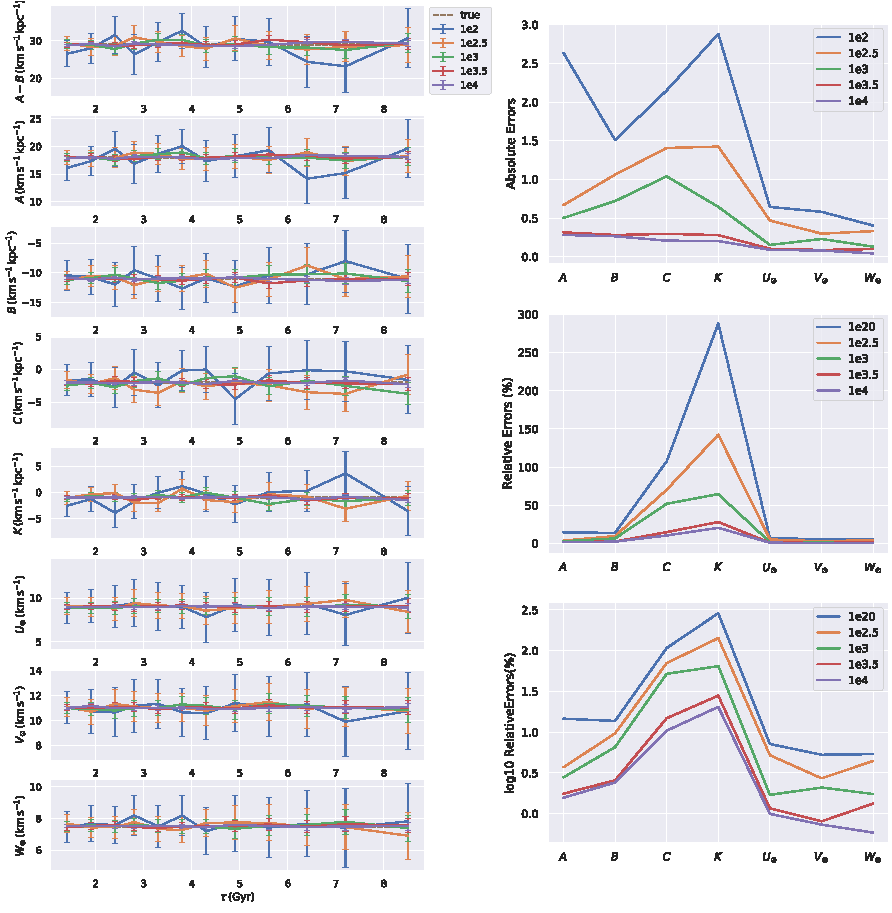
\includegraphics[width=15cm]{fig/Mock_N.pdf}
% 	\caption{解析6。サンプル数を変えて解析したときの結果の相対誤差。横軸は各パラメータ、縦軸は模擬データ生成時に設定した値と解析結果の値との相対誤差のlogスケール。サンプル数が多いほど相対誤差が小さくなっていることがわかる。左側の図は各パラメータごとの値。右側上図は相対誤差、右側下図は絶対誤差を表している。} \label{fig:Mock_N}
% \end{figure*}

%%%%%%%%%%%%%%%%%%%%%%%%%%%%%%%%%%%%%%%%%%%%%%%%%%%%%%%%%%%%%%%%%%%%%%%%%%%%%%%%%%%%%%%%%%%%%%%%
%%%%%%%%%%%%%%%%%%%%%%%%%%%%%%%%%%%%%%%%%%%%%%%%%%%%%%%%%%%%%%%%%%%%%%%%%%%%%%%%%%%%%%%%%%%%%%%%
%%%%%%%%%%%%%%%%%%%%%%%%%%%%%%%%%%%%%%%%%%%%%%%%%%%%%%%%%%%%%%%%%%%%%%%%%%%%%%%%%%%%%%%%%%%%%%%%

\subsection{解析6: $R_{\odot}$の値の解析結果への影響}
オールト定数と太陽運動の測定の先行研究では、仮定されている太陽と銀河中心との距離$R_{\odot}$がそれぞれの先行研究で異なる。この値はだいたい$\SI{7.5}{kpc}$から$\SI{8.5}{kpc}$の間であり、最大約10\%の違いがある。そこで、仮定する$R_{\odot}$の値が実際の$R_{\odot}$と異なる場合にどの程度測定値を間違うのかを調べることにした。

解析6では、模擬データAを解析する際に$R_{\odot}$の値を$R_{\odot} = 6.2、8.2、10.2\,\si{kpc}$と変えて3パターンで解析した。解析6ではasymmetric driftを考慮している。なぜなら、$R_{\odot}$はasymmetric driftを考慮する尤度関数 (式(\ref{Likelihood_Mock_AD}))を使用するときのみに影響するからである。具体的には、式(\ref{eq142})の上から2つ目の式と式(\ref{eq153})で$R_{\odot}$を使用する。一方、asymmetric driftを考慮しない尤度関数 (式(\ref{Likelihood_Mock}))では$R_{\odot}$の値は使用しない。

図\ref{fig:Mock_R0}は解析6の結果である。この図を見ると、$R_{\odot}=\SI{6.2}{kpc}、\SI{10.2}{kpc}$のときオールト定数$A、B$は大きく間違った値となっており、$R_{\odot}=\SI{8.2}{kpc}$のときのfit - trueが最も小さくなっていることがわかる。年齢依存性は確認できない。

\begin{figure*}[htbp]
	\centering
	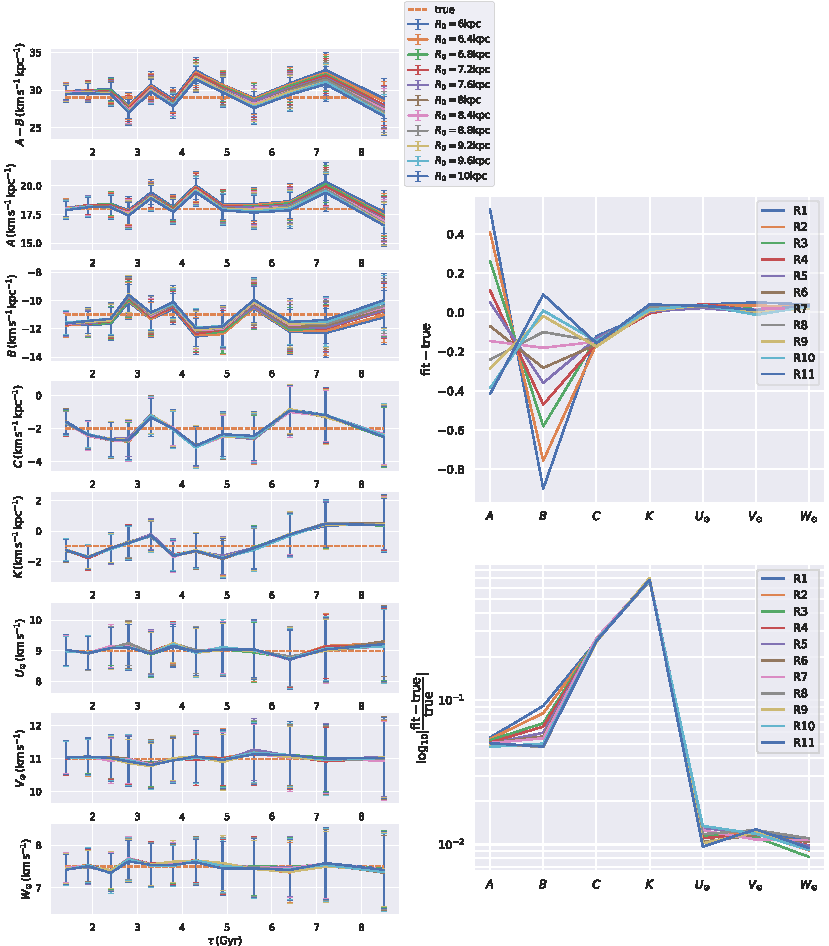
\includegraphics[width=15cm]{fig/Mock_R0.pdf}
	\caption{解析6。模擬データAを解析するときに太陽の銀河中心からの距離の仮定する値を$R_{\odot}$を$R_{\odot} = 6.2、8.2、10.2\,\si{kpc}$と変えて、asymmetric driftを考慮せずに解析した結果。縦軸は各パラメータのfit (解析で得られた値) - true (模擬データに設定した値)、横軸は模擬データに入れた速度分散に対応する年齢。} \label{fig:Mock_R0}
\end{figure*}